

\section{Introduction to RF and microwave integrated circuits}
\subsection{Define RF, microwaves and millimeter waves from the standpoint of frequency allocation.}
We distinguish based on the frequency:
\begin{enumerate}
    \item \textit{RF}:frequency between a few MHz and 1 GHz, free space wavelengths
    of the order of 1 m (es. long distance radar --> large wavelength, large microwave)
    \item \textit{Microwave}: frequencies between 1 GHz and 30 GHz, free space wavelengths
    between 30 cm and 1 cm. (es . clock frequency)    
    \item \textit{Millimiter waves}:  frequencies between 30 GHz and 100 (300) GHz, free space
    wavelengths below 1 cm. es automotive
\end{enumerate}


\subsection{ Suppose a radar has to be designed to detect objects of the average size of 1 cm: is an RF
operating frequency adequate to this? Explain why/why not. Suggest if the case a more suitable
frequency range.}
No it's not.


\subsection{Identify the L and the K bands (frequency limits). In what frequency band are GSM cellphones
operating?}
\begin{figure}[H]
    \centering
    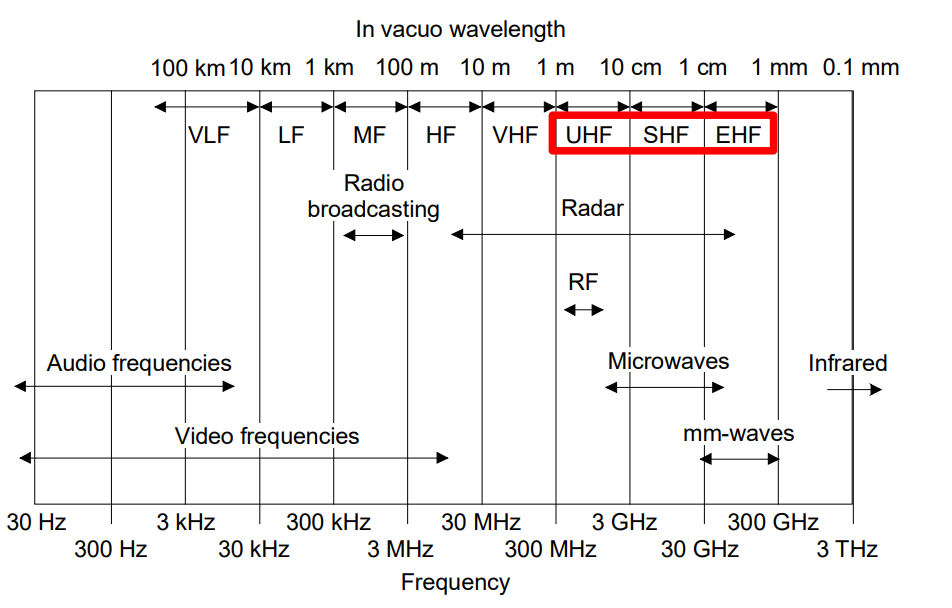
\includegraphics[width=0.6\textwidth]{pictures/cap1/bande.png}
    \caption{Frequency bands}
    \label{fig:mia_immagine}
\end{figure}


\subsection{Explain why signals cannot conveniently transmitted in baseband through a Hertzian channel,
but rather they have to be upconverted through analog or digital modulations. Assume as an
example e.g. a hi-fi signal with frequency between DC and 20 kHz.}


\subsection{ Explain why transmitting the human voice in baseband through a portable phone would be
for many reasons unpractical.}

\subsection{In a cellular system each cell exploits the same frequency bands (e.g. around 2 GHz). Explain
how there is no interference between di§erent users in the same cell and between nearby cells.}

\subsection{Describe a basic RF RX/TX (receiver/transmitter) scheme}

\begin{figure}[H]
    \centering
    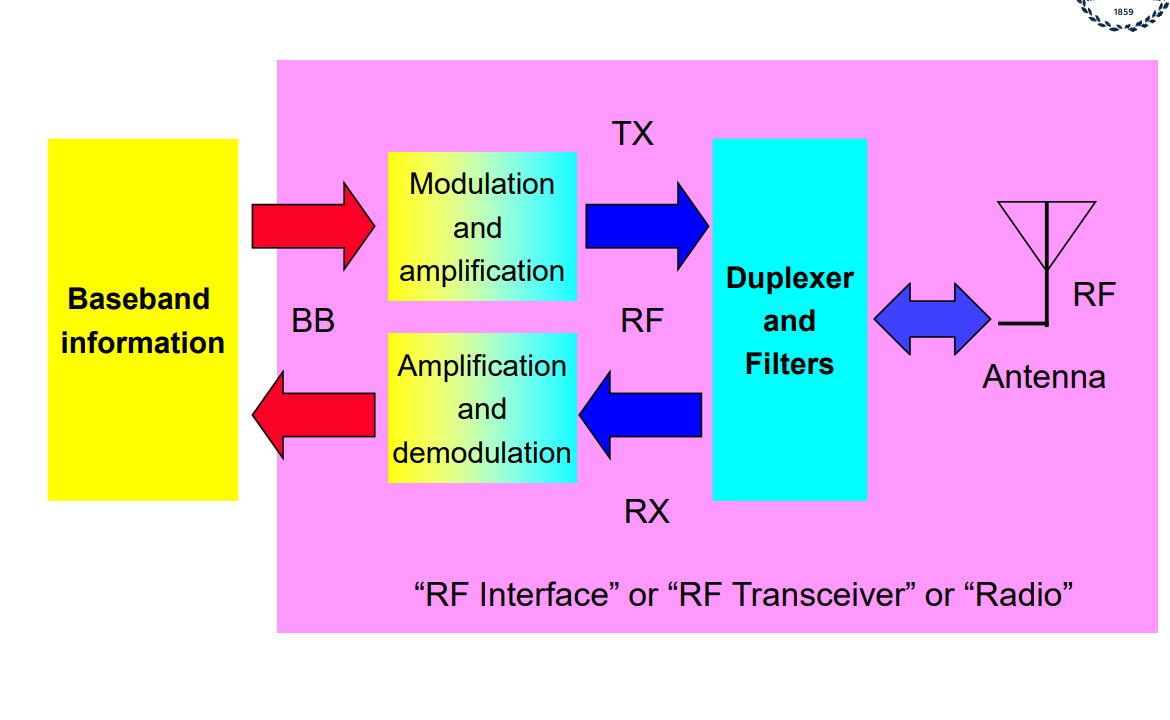
\includegraphics[width=0.6\textwidth]{pictures/cap1/blcok_scheme.png}
    \caption{Scheme}
    \label{fig:mia_immagine}
\end{figure}
Duplexer switches the antennna TX or RX

\subsection{ List the basic RX section building blocks, starting from the antenna down to the downconversion mixer}
\begin{figure}[H]
    \centering
    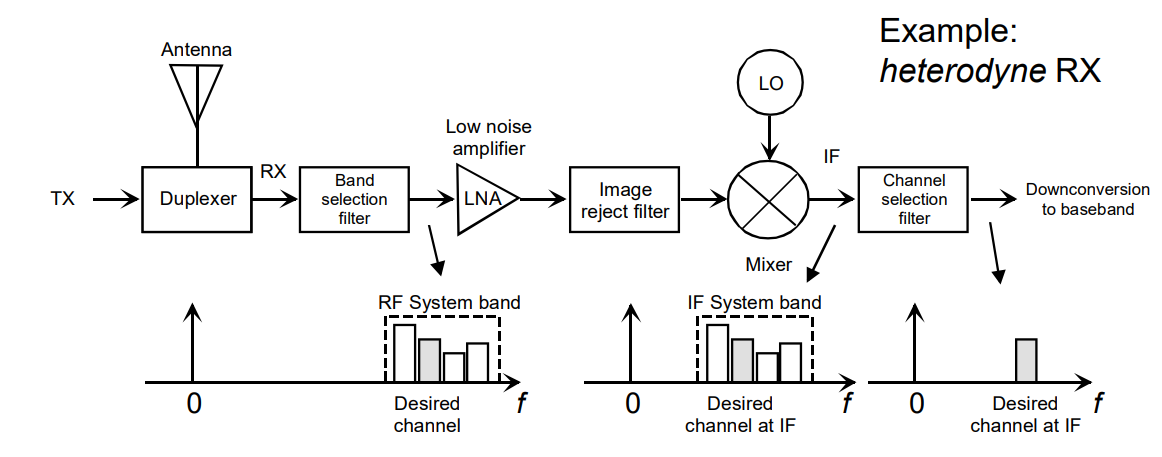
\includegraphics[width=0.6\textwidth]{pictures/cap1/Rx.png}
    \caption{Receiver scheme}
    \label{fig:mia_immagine}
\end{figure}
In ordere I have:
\begin{enumerate}
    \item \textit{band selection filter}: The band selection filter is bandpass filter that filter out everything outside the band. The amount of noise is proportional to the bandwidth , in addition
    I could have interferences and disturbances. I can't select the specific channel: I would need a very high selectivity filter (difficile) and fileter whose 
    bandwith change dinamically (??)
    \item \textit{LNA} : low noise amp, the greatest noise contribution comes from the first element(veder catena offset)
    \item \text{image rejection filter}
    \item \text{Mixer} heterodyne or homodyne: Desired channel at IF frequency 
    \item \text{Channel selection} 
\end{enumerate}

\subsection{List the basic TX section building blocks, starting from the upconversion mixer up to the
antenna}

\begin{figure}[H]
    \centering
    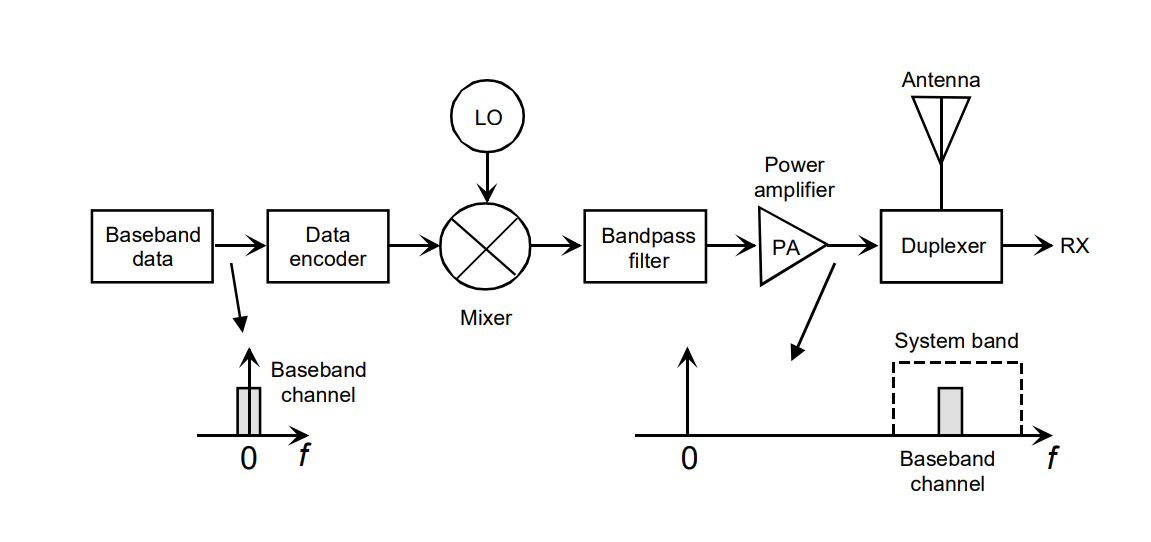
\includegraphics[width=0.6\textwidth]{pictures/cap1/Tx.png}
    \caption{Transmitter scheme}
    \label{fig:mia_immagine}
\end{figure}
\begin{itemize}
    \item \textit{Mixer}: modulate up
    \item \textit{PA}
\end{itemize}


\subsection{What is the difference between a homodyne ad a heterodyne receiver?}
Mixer is a bilinear component: the output is the product of the 2 inputs. I have the high and low frequency , up or down convertion
depends on the filter applied after. $\omega_{If}= \omega_{RF}-\omega_{LO}$ is called \textit{lows side injection} the other case is called \textit{high
side injection}

\begin{figure}[H]
    \centering
    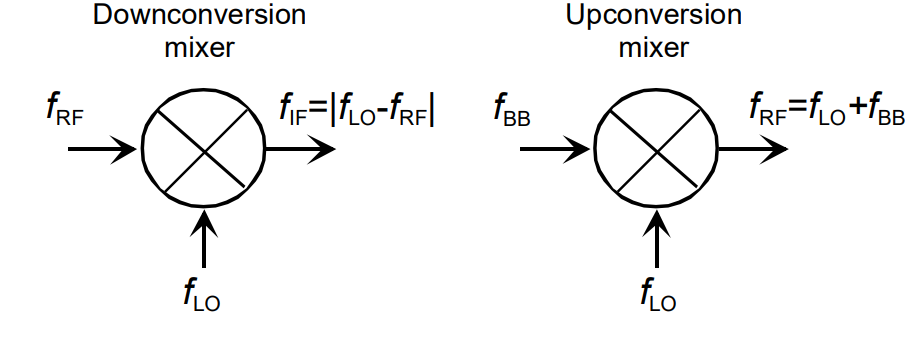
\includegraphics[width=0.6\textwidth]{pictures/cap1/mixer.png}
    \caption{Mixer}
    \label{fig:mia_immagine}
\end{figure}


In \textit{Heterodyne} I need a image rejection filter in case of downconversion I have aliasing (vedi meglio slide). The 
RX band is downconverted into Intermediate Frequency (IF) and relax the filter Q for channel selection. (2 steps)
In \textit{Heterodyne} the RX band is directly downconverted into Baseband also called Direct Conversion receivers. 
We immediately have the quadrature filter we eliminate the intermediate frequency 


\subsection{What is the difference between a low noise, high gain and maximum power amplifier?}
When we talk about amplfier usually is a cascaded multistage of more amps , we difine:
\begin{itemize}
    \item \text{Low noise amp}: the first stage is LNA the others are HGA. Being in a RX I don't need high power.
    \item \text{High gain}: all stages are HGA, linear design topology.
    \item \text{Power}:the last stage is PA (not high gain however 6 dB max , they are limited by distortion and others non linear stuff) by design, the others HGA.
\end{itemize}

  
\subsection{What are the typical features of planar vs. waveguide microwave circuits}
\begin{itemize}
    \item \textit{Waveguide}:big heavy and expensive but on the other hand high power and low losses. Still used such Radar
    \item \textit{Planar}: ow cost, small size, same approach as low-frequency ICs or hybrid circuits 

\end{itemize}

\subsection{ Explain the differences between a hybrid and a monolithic microwave circuit.}

\begin{itemize}
    \item \textit{Monolithic}: everything is integrated in a semiconductor substrate passive and active device
    \item \textit{Hybrid} passive device are generally integrated on suportive dieletric subrstrate while active are connected externally.
\end{itemize}
Hybrid is easier to prototype (PCB) , Monolithic very long and expensive.
\begin{figure}[H]
    \centering
    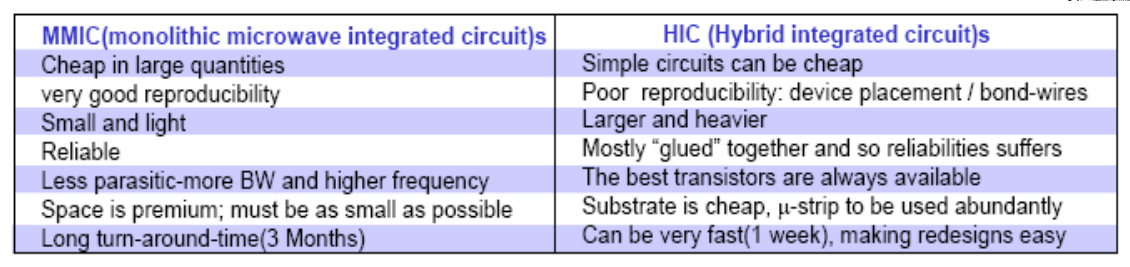
\includegraphics[width=0.6\textwidth]{pictures/cap1/monolitic.png}
    \caption{Differences between monolithic and hybrid}
    \label{fig:mia_immagine}
\end{figure}


\subsection{List in order of increasing frequency range the following semiconductors: indium phosphide,
silicon, gallium arsenide}
\begin{enumerate}
    \item InP - HEMTS up to mm waves
    \item GaAs - MESFET 50 GHz
    \item Silicon -MOS 20-30 GHz
\end{enumerate}

\subsection{Explain the difference between a lumped and a distributed-parameter circuit. Why distributed
elements cannot be integrated in an RF circuit?}
\begin{enumerate}

\item \textbf{Lumped parameter circuits} : inductor , resistor,Filters, Couplers, Lumped power divider .. used in monolithic
\begin{itemize}
    \item Elements are small compared to the wavelength 
    ($< \lambda/8$)
    \item Typically integrated on silicon substrate 
\end{itemize}

\item \textbf{Distributed parameter circuits}: Transmission lines, simple and coupled
\begin{itemize}
    \item Elements based on transmission line structures and  physical dimensions comparable with the wavelength 
    ($> \lambda/8$)
    \item Typically hybrid implementations:Active devices are discrete and passive elements integrated on the substrate 
        (or sometimes discrete lumped components). Circuits are fabricated on dielectric substrates 
    \item High-frequency integrated circuits often include 
    distributed elements
\end{itemize}
Distributed elements cannot easily be integrated in RF circuits because their dimensions are comparable to the wavelength, 
which is too large for ICs, and because silicon substrates introduce high losses and low-Q passive structures.
\end{enumerate}

\subsection{Quote a few microwave field-effect or bipolar transistors with the related semiconductor
material.}
\begin{itemize}
    \item Si-based Mosfet -field
    \item GaN based HEMTS -field
    \item InP based HEMTS - field
    \item Si based BJT
    \item SiGe HBTs
    \item  GaAs HBT
\end{itemize}

\subsection{Explain the difference between analog large-signal and small-signal models. Clarify what
model is linear and what model is nonlinear.}

\subsection{Explain the difference between a memoriless model and a model with memory.}